\documentclass{ximera}

\newcommand{\RR}{\mathbb R}
\renewcommand{\d}{\,d}
\newcommand{\dd}[2][]{\frac{d #1}{d #2}}
\renewcommand{\l}{\ell}
\newcommand{\ddx}{\frac{d}{dx}}
\newcommand{\dfn}{\textbf}
\newcommand{\eval}[1]{\bigg[ #1 \bigg]}


\begin{document}
\begin{problem}
  Compute the \textbf{volume} between the elliptic paraboloid $z = 9-x^2-y^2$
  and the $(x,y)$-plane.
  \begin{prompt}
    \[
    \text{volume} = \answer{81\pi/2}
    \]
  \end{prompt}
\end{problem}

\vfill
\hrule
\begin{problem}
  Use \textbf{any method} you like to compute:
  \[
  \int_{-3}^{3} \int_{-\sqrt{9-z^2}}^{\sqrt{9-z^2}}\int_{-5}^1 \d x\d y \d z
  \begin{prompt}
  =\answer{54\pi}  
  \end{prompt}
  \]
  \textbf{Give a very brief explanation.}
  \begin{feedback}[correct]
    This is the volume of a cylinder of radius $3$ and height $6$.
  \end{feedback}
  \vfill
\end{problem}
\hrule

\textbf{Problems 7 and 8} are related.
\begin{problem}
  \textbf{Sketch} the \textbf{region of integration} for the integral: $\int_0^1\int_x^{\sqrt{2-x^2}} \cos(x^2+y^2)\d y \d x$
  \begin{image}[2in]
    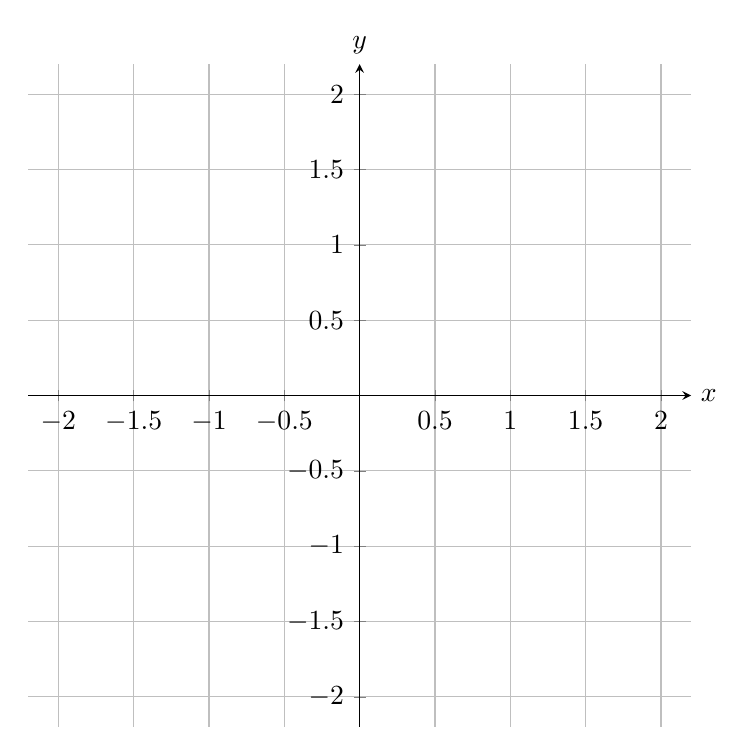
\begin{tikzpicture}
      \begin{axis}[
          xmin=-2.2,xmax=2.2,ymin=-2.2,ymax=2.2,
          clip=false,
          axis lines=center,
          width=10cm,
          height=10cm,
          xtick={-2,-1.5,...,2},
          ytick={-2,-1.5,...,2},
          xlabel=$x$, ylabel=$y$,
          grid = major,
          every axis y label/.style={at=(current axis.above origin),anchor=south},
          every axis x label/.style={at=(current axis.right of origin),anchor=west},
        ]
        %\addplot[very thick,black,->] plot coordinates {(1,1) (4,2)};
        %\addplot[very thick,black,->] plot coordinates {(-1,0) (-3,3)};
        %\node[above] at (axis cs:2.5, 1.5) {$\vec{w}$};
        %\node[above] at (axis cs:-2, 1.5) {$\vec{v}$};
      \end{axis}
    \end{tikzpicture}
  \end{image}
  \begin{prompt}
    \begin{multipleChoice}
        \choice[correct]{I've drawn this.}
    \end{multipleChoice}
    \begin{feedback}[correct]
        \begin{image}
          \includegraphics{scan3.jpg}
        \end{image}
      \end{feedback}
    \end{prompt}
\end{problem}


\begin{problem}
  \textbf{Compute:}  $\int_0^1\int_x^{\sqrt{2-x^2}} \cos(x^2+y^2)\d y \d x$
  \begin{prompt}
    \[
    = \answer{\frac{\pi\sin(2)}{8}}
    \]
  \end{prompt}
  \vfill
\end{problem}

\end{document}
